\documentclass[11pt]{article}

% ----- lightweight preamble (matches CICLink.tex / PatternMap.tex) -----
\usepackage[a4paper,margin=1.4cm]{geometry}
\usepackage{amsmath,amssymb}
\usepackage{tikz}
\usetikzlibrary{arrows.meta,positioning,calc,fit,backgrounds,
  shapes.geometric,chains,decorations.pathreplacing}
\usepackage[most]{tcolorbox}
\usepackage{parskip}
\usepackage{xcolor}

\definecolor{ink}{RGB}{40,40,40}
\definecolor{soft}{RGB}{245,245,248}
\definecolor{gen}{RGB}{30,110,190}   % generic  TransitionSystem
\definecolor{mux}{RGB}{30,140,80}    % MutexExample
\definecolor{tin}{RGB}{200,140,0}    % TinyTS
\definecolor{cic}{RGB}{170,60,60}    % CICLink / recursor
\definecolor{gd}{RGB}{30,140,80}     % good / conclusion

\newtcolorbox{note}[1][]{colback=soft,colframe=ink,boxrule=0.4pt,
  arc=2pt,left=6pt,right=6pt,top=4pt,bottom=4pt,#1}

\tikzset{
  box/.style={draw=ink,rounded corners=3pt,fill=soft,inner sep=5pt,
    font=\small,align=center},
  chip/.style={draw=ink,rounded corners=6pt,fill=soft,inner sep=6pt,
    font=\small\bfseries,align=center,minimum height=11mm},
  code/.style={draw=ink,rounded corners=2pt,fill=white,inner sep=4pt,
    font=\ttfamily\scriptsize,align=left},
  arr/.style={-{Stealth[length=2.8mm]},thick},
  eq/.style={{Stealth[length=2.2mm]}-{Stealth[length=2.2mm]},thick,ink},
  lbl/.style={font=\scriptsize\itshape,text=ink,align=center},
}

\title{\vspace{-1.6cm}\textbf{Base $+$ Step $\Rightarrow$ Forever}\\[2pt]
\large The honest core of certifying model checking, in pictures}
\author{\small \texttt{RequestProject/ModelChecking} ---
TransitionSystem $\cdot$ MutexExample $\cdot$ TinyTS $\cdot$ CICLink}
\date{}

\begin{document}
\maketitle
\vspace{-1.1cm}

\begin{note}
\textbf{One idea.} A property that is \emph{true at the start} and
\emph{kept by every step} is \emph{true forever}. That is the whole story.
We (a)~state it exactly, (b)~let Lean check it, and (c)~notice it is just Lean's
own induction rule. It is not a model checker --- it is the soundness ground
under one.
\end{note}

%=====================================================================
\section*{1. The pipeline (five words)}

\begin{center}
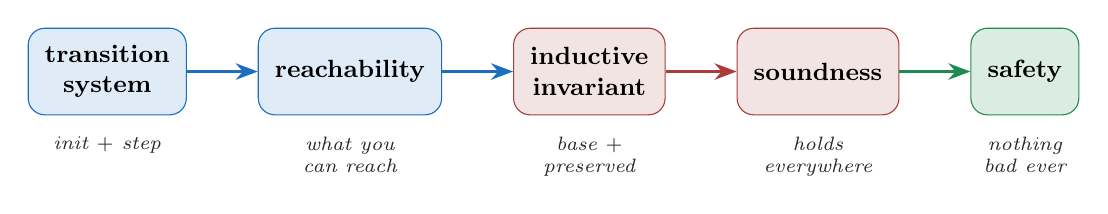
\begin{tikzpicture}[node distance=7mm]
  \node[chip,fill=gen!14,draw=gen] (ts) {transition\\system};
  \node[chip,fill=gen!14,draw=gen,right=9mm of ts] (rc) {reachability};
  \node[chip,fill=cic!14,draw=cic,right=9mm of rc] (inv) {inductive\\invariant};
  \node[chip,fill=cic!14,draw=cic,right=9mm of inv] (snd) {soundness};
  \node[chip,fill=gd!16,draw=gd,right=9mm of snd] (saf) {safety};
  \draw[arr,gen] (ts) -- (rc);
  \draw[arr,gen] (rc) -- (inv);
  \draw[arr,cic] (inv) -- (snd);
  \draw[arr,gd] (snd) -- (saf);
  \node[lbl,below=1.5mm of ts] {init $+$ step};
  \node[lbl,below=1.5mm of rc] {what you\\can reach};
  \node[lbl,below=1.5mm of inv] {base $+$\\preserved};
  \node[lbl,below=1.5mm of snd] {holds\\everywhere};
  \node[lbl,below=1.5mm of saf] {nothing\\bad ever};
\end{tikzpicture}
\end{center}

%=====================================================================
\section*{2. The picture behind it}

\begin{center}
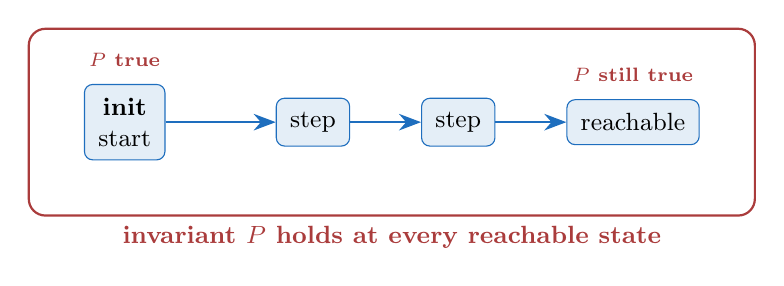
\begin{tikzpicture}[node distance=8mm]
  \node[box,fill=gen!12,draw=gen] (init) {\textbf{init}\\start};
  \node[box,fill=gen!12,draw=gen,right=14mm of init] (s1) {step};
  \node[box,fill=gen!12,draw=gen,right=9mm of s1] (s2) {step};
  \node[box,fill=gen!12,draw=gen,right=9mm of s2] (s3) {reachable};
  \draw[arr,gen] (init) -- (s1);
  \draw[arr,gen] (s1) -- (s2);
  \draw[arr,gen] (s2) -- (s3);
  \begin{scope}[on background layer]
    \node[fit=(init)(s3),draw=cic,thick,rounded corners=6pt,
      inner sep=7mm,label={[cic,font=\small\bfseries]below:%
      invariant $P$ holds at every reachable state}] {};
  \end{scope}
  \node[cic,font=\scriptsize\bfseries,above=1mm of init] {$P$ true};
  \node[cic,font=\scriptsize\bfseries,above=1mm of s3] {$P$ still true};
\end{tikzpicture}
\end{center}

\begin{center}\footnotesize
$P$ true at start \;$+$\; each step keeps $P$
\;$\Longrightarrow$\; $P$ true everywhere.
\end{center}

%=====================================================================
\section*{3. Four files, one shape}

\begin{center}
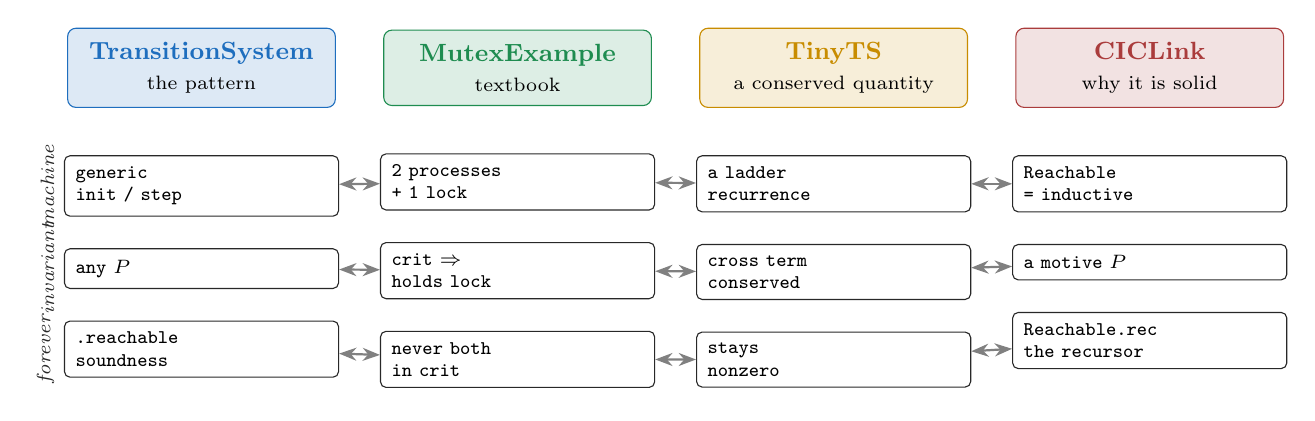
\begin{tikzpicture}[node distance=4mm]
  \node[box,fill=gen!15,draw=gen,minimum width=34mm] (h1)
    {\textcolor{gen}{\textbf{TransitionSystem}}\\\scriptsize the pattern};
  \node[box,fill=mux!15,draw=mux,minimum width=34mm,right=6mm of h1] (h2)
    {\textcolor{mux}{\textbf{MutexExample}}\\\scriptsize textbook};
  \node[box,fill=tin!15,draw=tin,minimum width=34mm,right=6mm of h2] (h3)
    {\textcolor{tin}{\textbf{TinyTS}}\\\scriptsize a conserved quantity};
  \node[box,fill=cic!15,draw=cic,minimum width=34mm,right=6mm of h3] (h4)
    {\textcolor{cic}{\textbf{CICLink}}\\\scriptsize why it is solid};

  \node[code,below=6mm of h1.south,anchor=north,text width=32mm] (c1) {generic\\ init / step};
  \node[code,below=6mm of h2.south,anchor=north,text width=32mm] (c2) {2 processes\\ + 1 lock};
  \node[code,below=6mm of h3.south,anchor=north,text width=32mm] (c3) {a ladder\\ recurrence};
  \node[code,below=6mm of h4.south,anchor=north,text width=32mm] (c4) {Reachable\\ = inductive};
  \node[lbl,left=0mm of c1,rotate=90,anchor=south] {machine};

  \node[code,below=4mm of c1.south,anchor=north,text width=32mm] (d1) {any $P$};
  \node[code,below=4mm of c2.south,anchor=north,text width=32mm] (d2) {crit $\Rightarrow$\\ holds lock};
  \node[code,below=4mm of c3.south,anchor=north,text width=32mm] (d3) {cross term\\ conserved};
  \node[code,below=4mm of c4.south,anchor=north,text width=32mm] (d4) {a motive $P$};
  \node[lbl,left=0mm of d1,rotate=90,anchor=south] {invariant};

  \node[code,below=4mm of d1.south,anchor=north,text width=32mm] (e1) {.reachable\\ soundness};
  \node[code,below=4mm of d2.south,anchor=north,text width=32mm] (e2) {never both\\ in crit};
  \node[code,below=4mm of d3.south,anchor=north,text width=32mm] (e3) {stays\\ nonzero};
  \node[code,below=4mm of d4.south,anchor=north,text width=32mm] (e4) {Reachable.rec\\ the recursor};
  \node[lbl,left=0mm of e1,rotate=90,anchor=south] {forever};

  \foreach \a/\b in {c1/c2,c2/c3,c3/c4,d1/d2,d2/d3,d3/d4,e1/e2,e2/e3,e3/e4}
    \draw[eq,gray] (\a) -- (\b);
\end{tikzpicture}
\end{center}

\begin{center}\footnotesize
\textcolor{gray}{$\longleftrightarrow$ each grey link $=$ ``same shape, different words''.}
\end{center}

%=====================================================================
\section*{4. The two examples, side by side}

\begin{center}
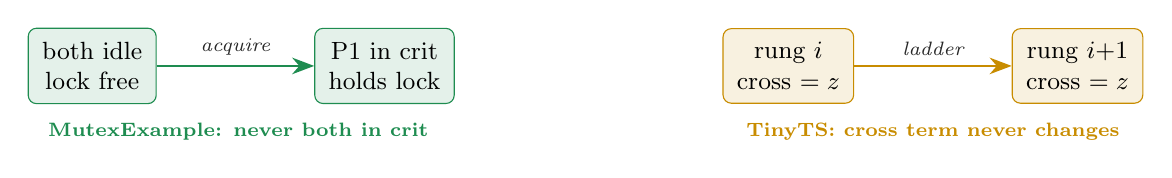
\begin{tikzpicture}[node distance=8mm]
  % mutex
  \node[box,fill=mux!12,draw=mux] (m0) {both idle\\lock free};
  \node[box,fill=mux!12,draw=mux,right=20mm of m0] (m1) {P1 in crit\\holds lock};
  \draw[arr,mux] (m0) -- node[lbl,above]{acquire} (m1);
  \node[mux,font=\scriptsize\bfseries,below=6mm of $(m0)!0.5!(m1)$]
    {\textcolor{mux}{MutexExample:} never both in crit};
  % tinyts
  \node[box,fill=tin!12,draw=tin,right=34mm of m1] (t0) {rung $i$\\cross $= z$};
  \node[box,fill=tin!12,draw=tin,right=20mm of t0] (t1) {rung $i{+}1$\\cross $= z$};
  \draw[arr,tin] (t0) -- node[lbl,above]{ladder} (t1);
  \node[tin,font=\scriptsize\bfseries,below=6mm of $(t0)!0.5!(t1)$]
    {\textcolor{tin}{TinyTS:} cross term never changes};
\end{tikzpicture}
\end{center}

%=====================================================================
\section*{5. The elegant part: soundness \emph{is} the recursor}

\begin{center}
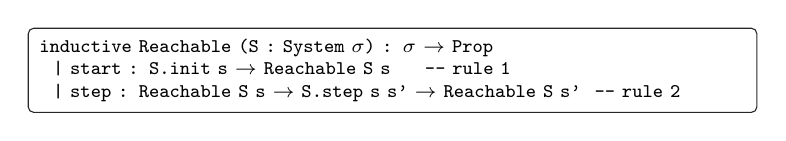
\begin{tikzpicture}
  \node[code,text width=0.74\linewidth] {
inductive Reachable (S : System $\sigma$) : $\sigma$ $\to$ Prop\\
\ \ | start : S.init s\ $\to$\ Reachable S s\ \ \ \ \ -- rule 1\\
\ \ | step\ : Reachable S s\ $\to$\ S.step s s'\ $\to$\ Reachable S s'\ \ -- rule 2
  };
\end{tikzpicture}
\end{center}

\begin{center}
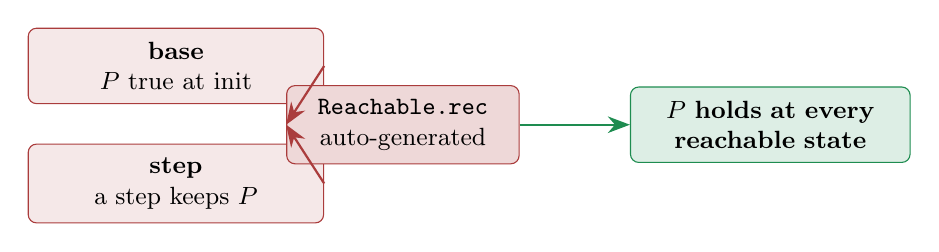
\begin{tikzpicture}[node distance=6mm]
  \node[box,fill=cic!12,draw=cic,text width=34mm] (a) {\textbf{base}\\ $P$ true at init};
  \node[box,fill=cic!12,draw=cic,text width=34mm,below=5mm of a] (b) {\textbf{step}\\ a step keeps $P$};
  \node[box,fill=cic!20,draw=cic,right=14mm of $(a)!0.5!(b)$,text width=26mm] (r)
    {\texttt{Reachable.rec}\\ auto-generated};
  \node[box,fill=gd!15,draw=gd,right=14mm of r,text width=32mm] (o)
    {\textbf{$P$ holds at every reachable state}};
  \draw[arr,cic] (a.east) -- (r.west);
  \draw[arr,cic] (b.east) -- (r.west);
  \draw[arr,gd] (r) -- (o);
\end{tikzpicture}
\end{center}

\begin{center}
\begin{note}[width=0.88\linewidth]
\centering\small
The two rules \emph{are} the two constructors. Lean auto-builds the recursor
\texttt{Reachable.rec}. Feed it the two invariant fields (base, step) and out
comes soundness. The \texttt{by induction} proof and the raw-recursor proof are
the \emph{same term} (checked by \texttt{rfl}), and it needs \emph{no} axioms.
\end{note}
\end{center}

%=====================================================================
\section*{6. What this is --- and is not}

\begin{center}
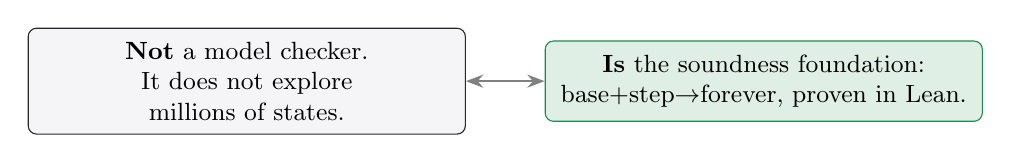
\begin{tikzpicture}[node distance=6mm]
  \node[box,fill=soft,draw=ink,text width=52mm] (no)
    {\textbf{Not} a model checker.\\ It does not explore millions of states.};
  \node[box,fill=gd!14,draw=gd,text width=52mm,right=10mm of no] (yes)
    {\textbf{Is} the soundness foundation:\\ base$+$step$\to$forever, proven in Lean.};
  \draw[eq,gray] (no) -- (yes);
\end{tikzpicture}
\end{center}

\begin{center}\footnotesize
Real tools scale this to millions of states $+$ SMT. Here it is small on
purpose --- so the core is fully understood and machine-checked.
\end{center}

%=====================================================================
\section*{One sentence}

\begin{center}
\begin{tcolorbox}[colback=soft,colframe=ink,width=0.92\linewidth,arc=3pt]
\centering
A property true at the start and preserved by every step is true forever ---
stated exactly, machine-checked in Lean, and revealed to be nothing more than
the inductive recursor.
\end{tcolorbox}
\end{center}

\begin{center}\footnotesize
All four files build with \texttt{lake build}, no \texttt{sorry}; the recursor
proof uses \emph{no} axioms.
\end{center}

\end{document}
